\documentclass{beamer}
\usetheme{focus}

\usepackage{subcaption}

\title{Bachelorarbeit\\ Abschlusspräsentation}
\subtitle{Suche von Einzelexemplaren}
\author{Pascal Baumann, Dane Wicki}
\begin{document}
\begin{frame}[plain]
    \maketitle
\end{frame}
\begin{frame}{Einleitung}
\end{frame}
\begin{frame}{Recap Zwischenpräsentation}
\begin{itemize}
    \item Kunde
    \item Aufgabenstellung und Ziele
    \item Referenzimplementation
    \item Konzepte
    \item Herausforderungen
\end{itemize}
\end{frame}
\begin{frame}{Impressionen Zwischenpräsentation}
\begin{figure}
    \centering
    \begin{subfigure}{0.45\linewidth}
        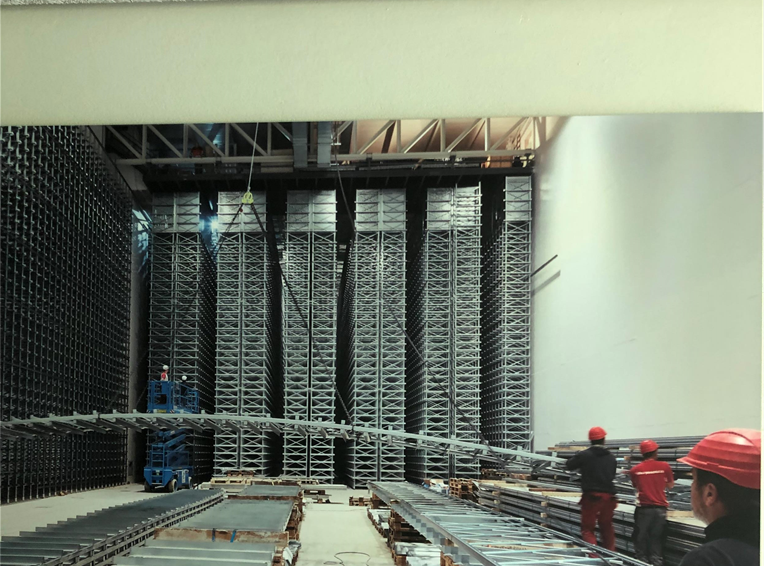
\includegraphics[width=0.8\linewidth]{img/Hochregallager}
    \end{subfigure}
    \begin{subfigure}{0.45\linewidth}
        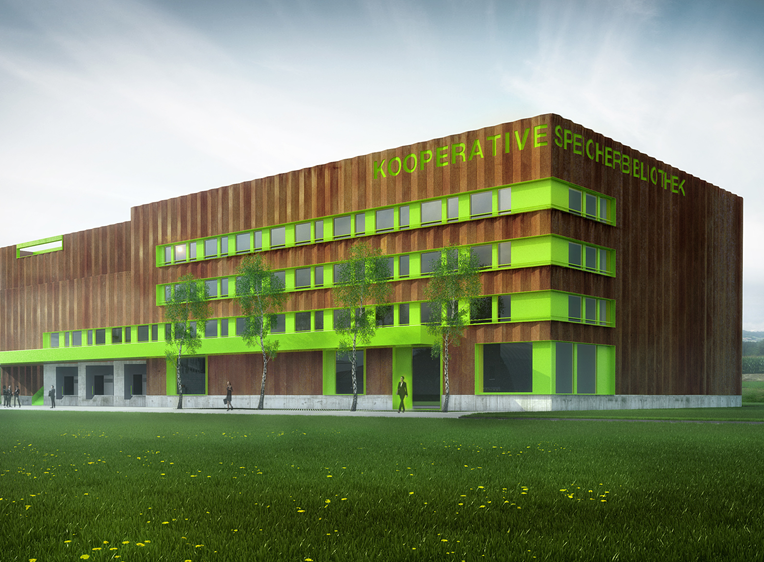
\includegraphics[width=0.8\linewidth]{img/Speicherbibliothek}
    \end{subfigure}
    \vspace{5em}
    \begin{subfigure}{0.7\linewidth}
        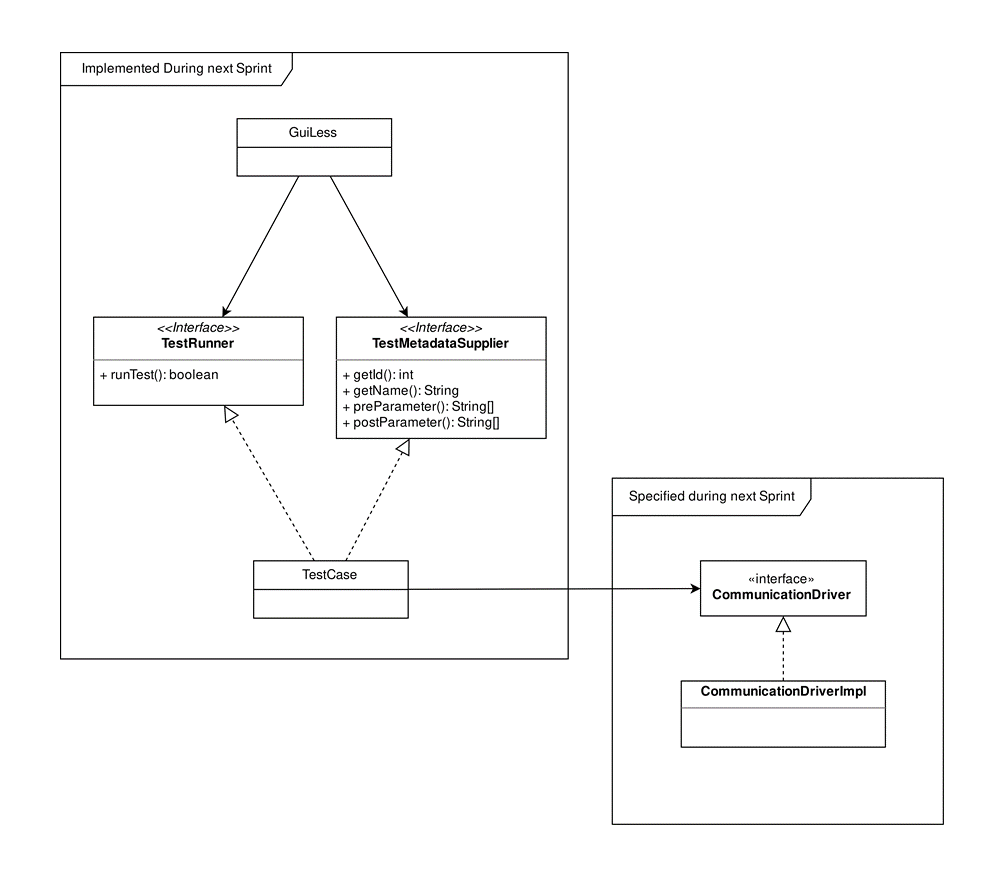
\includegraphics[width=0.7\linewidth]{img/Testframework}
    \end{subfigure}
\end{figure}
\end{frame}
\end{document}
